\documentclass[10pt]{article}
\usepackage[paperwidth=8.5in,paperheight=11in,left=0.9in,right=0.9in,top=0.85in,bottom=0.9in]{geometry}
\usepackage{multicol}
\usepackage{mathptmx}
\usepackage{amsmath,amssymb}
\usepackage{graphicx}
\usepackage{booktabs}
\usepackage{float}
\usepackage{caption}
\usepackage{titlesec}
\usepackage{fancyhdr}
\usepackage{tikz}
\usetikzlibrary{arrows.meta,positioning}
\usepackage[hidelinks]{hyperref}

\captionsetup{font=small,labelfont=sc,labelsep=period,justification=justified,singlelinecheck=false,skip=4pt}
\renewcommand{\figurename}{Fig}
\renewcommand{\tablename}{Table}
\renewcommand{\thetable}{\Roman{table}}
\titleformat{\section}{\normalfont\bfseries\large}{\Roman{section}.}{0.6em}{\MakeUppercase}
\titleformat{\subsection}{\normalfont\bfseries\itshape}{\Alph{subsection}.}{0.5em}{}
\titlespacing{\section}{0pt}{1.1ex plus .3ex}{0.6ex}
\titlespacing{\subsection}{0pt}{0.9ex plus .2ex}{0.4ex}
\setlength{\columnsep}{0.28in}
\setlength{\parskip}{0pt}
\setlength{\parindent}{10pt}
\renewcommand{\baselinestretch}{0.97}
\pagestyle{fancy}
\fancyhf{}
\fancyhead[C]{\thepage}
\renewcommand{\headrulewidth}{0pt}

\newcommand{\All}{\ensuremath{\mathrm{AllParticles}}}
\newcommand{\Perf}{\ensuremath{\mathrm{PerfectReco}}}

\begin{document}

\begin{center}
{\LARGE\bfseries Where inclusive beauty-hadron reconstruction loses chains:\\[2pt] geometry-aware inputs and the output form\par}
\vspace{0.9em}
{\large Q.~Guo\par}
\vspace{0.35em}
{\small University of Chinese Academy of Sciences, Beijing 100049, China\par}
\end{center}

\vspace{0.3em}
\begin{center}
\begin{minipage}{0.84\textwidth}
Reconstruction of beauty-hadron decays in the LHCb upgrade must run in real time on events with up to a thousand tracks. Deep full event interpretation (DFEI) represents an event as a graph of track pairs, prunes the graph with two graph neural networks, classifies each surviving pair by its lowest common ancestor generation (LCAG), and assembles decay chains from the classified graph. We measure where this chain efficiency is lost. On a fixed sample of 13\,255 signal chains, moving the cut on the pruning score raises the efficiency from 14.5\% to 17.9\% without retraining, and three features computed from the two track trajectories raise the intermediate 22.6\% model to 26.0\%. A pairwise ranking term adds 2.6 points at the new working point; six edge-context inputs and one round of attention on the line graph add 1.0 point each, the latter only when the pair geometry enters the attention logits. The efficiency reaches 28.0\%. We argue that the remaining loss is in the output form: an edge class followed by connected components carries no track-level background label and cannot enforce an exclusive assignment, which is the direction of current work.
\end{minipage}
\end{center}

\vspace{0.5em}
\begin{multicols}{2}

\section{Introduction}

The LHCb experiment will operate at a luminosity ten times the design value in Upgrade II, with up to fifty proton-proton collisions per bunch crossing and a charged-track multiplicity of order $10^3$ per event \cite{upgrade2}. Storing every event is not possible, and selecting events by reconstructing predefined candidates does not scale to the tens of thousands of decay modes of interest. Inclusive strategies instead interpret the event as a whole and retain the parts that belong to a heavy-flavour decay.

Deep full event interpretation (DFEI) is one such strategy \cite{dfei,hgnn}. Charged tracks are the nodes of a graph and every pair of tracks is a candidate edge. A node-pruning network removes tracks that are inconsistent with a $b$-hadron decay; an edge-pruning network removes pairs that are unlikely to belong to the same decay chain; a third network assigns each surviving pair an LCAG class, which encodes the generation of the shared ancestor for classes 0--3. Chains are defined as the connected components of the pairs with LCAG $>0$ (Fig.~\ref{fig:pipe}).

\begin{figure}[H]
\centering
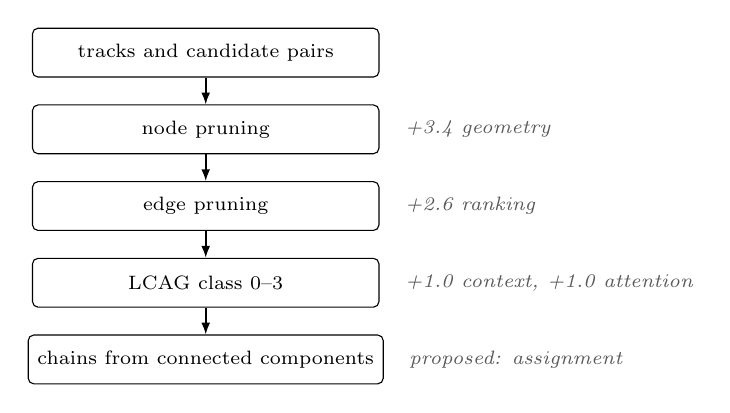
\begin{tikzpicture}[font=\scriptsize, node distance=3.4mm,
  box/.style={draw, rounded corners=2pt, minimum width=4.4cm, minimum height=6.2mm, align=center, fill=white},
  lab/.style={font=\scriptsize\itshape, text=black!65, align=left},
  arr/.style={-{Latex[length=1.5mm]}, semithick}]
\node[box] (a) {tracks and candidate pairs};
\node[box, below=of a] (b) {node pruning};
\node[box, below=of b] (c) {edge pruning};
\node[box, below=of c] (d) {LCAG class 0--3};
\node[box, below=of d] (e) {chains from connected components};
\draw[arr] (a)--(b); \draw[arr] (b)--(c); \draw[arr] (c)--(d); \draw[arr] (d)--(e);
\node[lab, right=2mm of b] {+3.4 geometry};
\node[lab, right=2mm of c] {+2.6 ranking};
\node[lab, right=2mm of d] {+1.0 context, +1.0 attention};
\node[lab, right=2mm of e] {proposed: assignment};
\end{tikzpicture}
\caption{Pipeline of DFEI and the places where this round adds information. The numbers are single-variable gains in percentage points of the fixed denominator and are not additive.}
\label{fig:pipe}
\end{figure}

This Letter reports where the chain efficiency is lost in that pipeline and what has to be added to move it. The study uses a simulated inclusive $b\bar b$ sample with a fixed denominator of 13\,255 signal chains, corresponding to 6089 test events and 2.18 chains per event. We quote efficiencies, not yields. \All{} is the fraction of signal chains whose reconstructed cluster contains exactly the truth tracks and no others; \Perf{} additionally requires the LCAG values of all pairs inside the cluster to agree with the truth. Both are quoted in percent of the fixed denominator. Statistical errors from this denominator are $\pm0.3$ percentage points at the 28\% level for a single number and $\pm0.4$ for a difference; training variance is not included, since all entries come from single runs.

The main observations are as follows. (i) The largest single change in this round is not a model change: it is the cut on the pruning scores, worth 3.5 points. (ii) Three features computed from the two track trajectories add 3.4 points to the 22.6\% intermediate model. (iii) A pairwise ranking term, matched to the thresholded use of the score, adds 2.6 points at the new working point. (iv) Six edge-context inputs add 1.0 point; one round of attention on the line graph adds a further 1.0 point, but attention alone is neutral and the gain requires the pair geometry in the attention logits. (v) The efficiency reaches 28.0\%, and the remaining loss is tied to the output form: an edge class followed by connected components has no track-level background label and cannot enforce an exclusive assignment.

\section{Method}

\subsection{Graph, pruning and assembly}

An event is represented by a heterogeneous graph with tracks and primary vertices (PVs) as node types. Track nodes carry kinematic and impact-parameter information and the associated PV. A track pair carries twelve inputs: $\Delta R$, $\Delta z$, the sum of charges, $\Delta p_T$, $\Delta$IP, a rank variable, DOCA and derived quantities. A node-pruning MLP scores each track and an edge-pruning MLP scores each pair; a pair is kept when both scores exceed their thresholds. The surviving pairs are classified into LCAG 0--3, and chains are the connected components of the pairs with a positive class. The baseline uses a threshold of 0.90 on both scores. It is trained with a binary cross-entropy whose positive weight is about 700, reflecting the signal fraction of roughly 0.14\% among candidate pairs, with AdamW, a batch size of eight, a learning rate of $10^{-4}$ and 30 epochs. The network has four graph blocks with 128--128--16 MLPs and a 16-dimensional latent space.

\subsection{Changes studied in this round}

Five changes are studied: four affect the score and one the output. (a) The cut on the node and edge scores moves from 0.90 to 0.95. (b) Three vertex-geometry features are added per pair: $\mathrm{DOCA}/100$, $\log(\mathrm{DOCA})$ and $|\Delta \mathrm{start}|/100$, where $\Delta\mathrm{start}$ is the three-dimensional distance between the two production vertices, in mm. The first two are recomputed locally because the stored column is affected by the sign error discussed in the Supplemental Material. (c) A pairwise ranking term is added to the edge loss; every signal edge is compared with the 64 highest-scoring background edges of the same event,
\begin{equation}
L_{\mathrm{rank}}=\big\langle \max(0,\ \tau+s_{\mathrm{bkg}}-s_{\mathrm{sig}})\big\rangle,\qquad \tau=1,
\end{equation}
with weight 10 in $L=L_{\mathrm{BCE}}+10\,L_{\mathrm{rank}}$; $s$ denotes the pruning logit, which is unbounded. (d) Six edge-context inputs are added. (e) Attention operates on the line graph of candidate pairs: pairs become nodes, neighbours are pairs that share a track in the same event, and the neighbourhood is truncated to 32 pairs. One round of four-head attention with 8 dimensions per head is applied after the last graph block, with a residual connection; a small network maps the pair geometry to a bias on the attention logits.

For the edge-context inputs, let $C(t)$ be the set of candidate pairs attached to track $t$. With $d_3$ the distance between the two production vertices in mm and $A=\exp(-d_3/50)$, one defines at each end of a pair $e=(i,j)$
\begin{equation}
\begin{aligned}
r_t&=\frac{A_e}{\max_{f\in C(t)}A_f},\quad
d_t=\frac{\#\{f\in C(t): A_f>0.5\}}{10},\\
c_t&=\frac{|C(t)|}{50}.
\end{aligned}
\end{equation}
The six inputs are the minimum and maximum of $r$, $d$ and $c$ over the two ends, which makes the vector symmetric under exchange of $i$ and $j$; the mother-daughter direction is not reliable at this stage. The scale of 50~mm is of the order of $c\tau_b$, so $A$ separates pairs from a common decay vertex from random pairs. The two counts differ: $d$ counts only pairs with $A>0.5$, whereas $c$ counts all candidates of the track. The edge vector grows from 12 to 18 columns, and the new columns start at zero so that the previous model is recovered at initialisation.

\section{Results}

\subsection{The cut}

Figure~\ref{fig:thr} shows the efficiency for the baseline weights at three cuts. At 0.90, 0.95 and 0.97 the values of \All{} are 14.5\%, 17.9\% and 18.5\%, and those of \Perf{} are 9.5\%, 11.7\% and 11.9\%. The gain of 3.5 points at 0.95 involves no retraining: it is a choice of where to cut. All numbers below use 0.95. Because the working point is a hyperparameter, the gain is realised only if the cut can be calibrated on data, which for a trigger would require a dedicated control sample; the quoted value is therefore an upper bound for a trigger application.

\begin{figure}[H]
\centering
\includegraphics[width=\columnwidth]{figs/thr.png}
\caption{\All{} (left bar of each pair) and \Perf{} (right bar) for the baseline weights at three cuts on the pruning scores. No retraining is involved.}
\label{fig:thr}
\end{figure}

\subsection{Vertex geometry}

The two DOCA features are recomputed from the track states: the stored column comes from an expression with a sign error, and its correlation with the recomputed value is 0.019, so it behaves as noise. The third feature, $|\Delta \mathrm{start}|$, is a new absolute quantity; the older derived block contained only $d_\perp/(|\Delta z|+1)$, which removes the overall scale. With the three features the efficiency moves from 22.6\% to 26.0\% and \Perf{} from 14.8\% to 17.8\% (Fig.~\ref{fig:vertex}). The three features enter together, so the gain cannot be split further; there is no run with $|\Delta \mathrm{start}|$ alone. Replacing only the stored DOCA column changes the efficiency from 14.5\% to 14.3\%: the corrected distance is useful only when supplied together with the two additional geometry features.

\begin{figure}[H]
\centering
\includegraphics[width=0.92\columnwidth]{figs/doca.png}
\caption{\All{} and \Perf{} before and after the three vertex-geometry features are added to the 22.6\% model.}
\label{fig:vertex}
\end{figure}

\subsection{Ranking term}

The positive weight of the BCE lifts signal edges but leaves their order against a background edge unconstrained, while the reconstruction thresholds the score. The pairwise term of Eq.~(1) is added for this reason. At the original cut it changes \All{} from 14.5\% to 16.3\%, and at 0.95 from 17.9\% to 20.5\%; \Perf{} changes from 9.5\% to 11.1\% and from 11.7\% to 13.6\%. Since only the relative order enters, the absolute score drifts and the working point has to be re-scanned.

\subsection{Edge context}

With the six inputs of Eq.~(2) the efficiency moves from 26.0\% to 27.0\%. At 0.90, where the comparison with the previous step is made, the number of retained background edges falls by 16\% while the number of retained signal edges falls by 3\%, so the purity of the kept edges rises from 11.6\% to 13.1\%. The global average precision of the edge score falls from 0.325 to 0.314: the gain is concentrated on nearly degenerate pairs, the region that determines whether a chain survives, whereas the global average is dominated by easily separated pairs.

\subsection{Attention}

Attention on the line graph takes the efficiency from 27.0\% to 28.0\%. On the earlier 21.8\% base, attention alone, without a geometric bias, is neutral (21.8\% to 21.6\%), and a bias built from $\Delta R$, $\Delta$IP and $\Delta z$ lowers it to 21.3\%. The gain appears only when the vertex geometry of the pair enters the attention logits,
\begin{equation}
\begin{aligned}
s_{ef}&=\frac{q_e\cdot k_f}{\sqrt{8}}+b_{ef},\\
b_{ef}&=\mathrm{MLP}\big([b_e,b_f,|b_e-b_f|,b_e\cdot b_f]\big),
\end{aligned}
\end{equation}
with $b_e$ containing DOCA, $\log$DOCA and $|\Delta\mathrm{start}|$. There is no run with the bias but without attention, so we conclude only that the pair geometry must enter the score; nothing here shows that attention itself is responsible for the gain.

\begin{figure}[H]
\centering
\includegraphics[width=\columnwidth]{figs/dist_m3.png}
\caption{Edge-score distribution before and after the attention step, for background (grey) and signal (green) pairs. The cut is at 0.90 in this figure; the efficiency numbers quoted in the text use 0.95.}
\label{fig:d3}
\end{figure}

\subsection{Small items and the ledger}

Table~\ref{tab:items} collects the single-variable changes and Fig.~\ref{fig:ledger} shows their cumulative effect. Five of them are at or below 0.8 points, and one entry, the minIP canonicalisation, is below the 0.4-point resolution of a single difference. Two further modules were tried and removed: an event-count auxiliary head cost 2.8 percentage points of efficiency and a PV-overlap input cost 0.4. The 22.6\% intermediate used above contains the cut, the ranking term, the change of checkpoint, and the three small input items; its composition is $17.9+2.6+0.8+0.8+0.5+0.2\approx22.8$, so the individual effects overcount the measured 22.6\% by about 0.2 points. This is why the entries are not additive.

\begin{table}[H]
\centering
\caption{Single-variable changes in percentage points of the fixed denominator. The second column gives the efficiency from which each change was measured. Statistical errors are $\pm0.4$ on a difference, so entries with $|\Delta|<0.4$ are not significant.}
\label{tab:items}
\footnotesize
\setlength{\tabcolsep}{4pt}
\begin{tabular}{lccc}
\toprule
Change & from & $\Delta$\All{} & $\Delta$\Perf{} \\
\midrule
Cut 0.90 $\rightarrow$ 0.95 & 14.5 & $+3.5$ & $+2.2$ \\
Ranking term & 17.9 & $+2.6$ & $+1.9$ \\
Checkpoint on pruning AP & 21.8 & $+0.8$ & $+0.3$ \\
Derived and triangle inputs & 14.5 & $+0.8$ & $+0.5$ \\
Event bias & 14.5 & $+0.5$ & $+0.6$ \\
minIP canonicalisation & 14.5 & $+0.2$ & $+0.3$ \\
Vertex geometry (3 features) & 22.6 & $+3.4$ & $+3.0$ \\
Edge context (6 inputs) & 26.0 & $+1.0$ & $+0.4$ \\
Attention with geometric bias & 27.0 & $+1.0$ & $+0.9$ \\
\bottomrule
\end{tabular}
\end{table}

\begin{figure}[H]
\centering
\includegraphics[width=\columnwidth]{figs/decomp.png}
\caption{Composition of the signal chains at each stage: removed by pruning (light grey), reconstructed with extra tracks (green), reconstructed exactly (blue). The first step contains the cut and the small items of Table~\ref{tab:items}.}
\label{fig:ledger}
\end{figure}

\section{Discussion}

The chain efficiency is limited not by the capacity of the graph network but by the information available to the score and by the position of the cut. Moving the cut alone gains 3.5 percentage points without retraining; three geometric features add 3.4 to the intermediate model; a ranking term matched to the thresholded use of the score adds 2.6. The two structural additions, edge context and attention, add one point each, and for the attention the control runs do not establish that the message passing itself is responsible.

Three caveats qualify these numbers. The sample is simulated and no systematic uncertainty is evaluated; the differences are from single training runs, so values below 0.4 points are not resolved. The working point was chosen on the same sample used for the quoted efficiency, which makes the 3.5-point entry an upper bound for a calibrated trigger. The gains are measured one at a time from the starting points of Table~\ref{tab:items} and do not add up.

Two controls are still missing and are the subject of the next round. A bias-only run, with the geometric bias added outside the attention, would separate the effect of the extra capacity from that of the message passing; and an equal-capacity MLP applied to the pair representation would test whether the gain requires the graph structure at all. Until those runs exist, the attention result should be read as an upper bound on what the geometry-in-score idea can deliver.

The numbers are for one simulated sample and one multiplicity regime. Neither the dependence on the number of tracks or PVs, nor the inference latency, has been measured here; the neighbourhood in the attention is truncated to 32 pairs, which keeps the cost linear in the number of candidate pairs, but a trigger-level timing study remains to be done.

The remaining loss is tied to the output. The current pipeline assigns a class to each pair and builds chains from connected components; this partition carries no track-level background label, and it cannot express the exclusivity between two candidate chains that compete for the same track, because the classes are defined per edge rather than per track. The natural object is therefore a partition of the tracks, trained with a partition-level objective: each track is assigned to at most one chain, or to background. Object condensation \cite{oc} and slot attention \cite{slot} are the two implementations being commissioned. The earlier attempt produced results identical to the baseline because of three implementation defects, which are documented in the Supplemental Material; corrected versions are being retrained, and no result is claimed here.

\vspace{0.4em}
\noindent\emph{Acknowledgments.} The author thanks the DFEI group for discussions and for access to the simulated samples and training infrastructure.

\vspace{0.3em}
\noindent\emph{Data and code availability.} The data and code underlying this Letter are available from the author on reasonable request.

\begin{thebibliography}{9}
\footnotesize
\bibitem{upgrade2} A.~Cerri \textit{et al.}, arXiv:1808.08865.
\bibitem{dfei} W.~Sutcliffe \textit{et al.}, arXiv:2504.21844.
\bibitem{hgnn} M.~Barbieri \textit{et al.}, arXiv:2610.16021.
\bibitem{oc} J.~Kieseler, arXiv:2002.03605.
\bibitem{slot} F.~Locatello \textit{et al.}, arXiv:2006.15055.
\end{thebibliography}

\end{multicols}
\end{document}
